% ============================================================
% back.tex -- Sections 6--9 (Integrative Discussion, MLP Agenda,
% Limitations, Conclusion). Every number is taken from
% raw_materials/experimental_log.md; model constants in Section 7
% are the canonical v1.0 specification in raw_materials/idea.md (Sec. 7).
% ============================================================

\section{Integrative Discussion}
\label{sec:discussion}

\subsection{What the three data lines jointly show}
\label{sec:discussion_lines}

A \emph{data line} is an evidentially separate source of relational data. The paper draws on three: (i) the literature corpus of Study~1 (E1), which records co-occurrence of AI and decision functions in documents and, in the network lines V6--V11.1, citation and co-authorship ties; (ii) six public organisational and relational sources screened for flow validity (E2; Section~\ref{sec:design}); and (iii) US utility patents, analysed at the domain, cell and firm levels in Study~2 (E3). Only the third line supplies directed dyadic flows between actors with externally assigned group labels, which is what Burt's construct requires \citep{burt1992structural} and what patent citations have long been used to approximate \citep{jaffe1993geographic}. The three patent analyses share one source and are therefore not independent replications of one another.

Read together, the lines support four statements. First, at the domain level AI and decision technologies are over-connected rather than separated: applicant citations between them occur at about three times the time-stratified expectation (OE $=3.05$, 95\% CI 2.94--3.17). Both relative criteria fail, and the verdict \texttt{HOLE\_NOT\_SUPPORTED} holds in all six preregistered sensitivity specifications (0/6 disagree). The over-connection is declining (WLS slope $-0.097$ per year, 95\% CI $-0.130$ to $-0.065$), but the last-three-year OE of 2.69 remains well above the reference median of 1.095, and the preregistered label is \texttt{PERSISTENT} (Figure~\ref{fig:patent_trend}).

Second, inside this over-connected pair the cell-level depletions are small and time-unstable. Apart from the quantum-computing cell (74 edges in Part~A), the cells depleted in both co-classification and citation flow have O/E between 0.70 and 0.95 (Figure~\ref{fig:cpc_heatmap}), and 0 depleted cells replicate across time halves (E3.3, P3).

Third, at the firm level specialist AI and decision firms are tied less than expected (O/E 0.24), but a null that preserves every firm's portfolio reproduces 85\% (primary) and 91\% (S-tech) of that separation. Mixed-portfolio firms are \emph{more} constrained than under the null (median constraint 0.358 against null medians of 0.104 and 0.116; $p=1.000$), so they show no brokerage advantage. The preregistered verdict is \texttt{PARTIAL} in both stratifications (Figure~\ref{fig:firm_null}).

Fourth, no data line confirms a Burt structural hole. The Study~1 network lines found 0 confirmed brokers (HISTORICAL / USER\_REPORTED; E1.6); no public source passed the independent-relation and validation gates, and the CORDIS bipartite null found 0 significant candidates (E2).

These results can appear to conflict with Study~1, where all 16 depleted function pairs remain depleted in both periods ($p=.86$ for the change against a permutation null). The two statements concern different units and references. Study~1 asks which \emph{function pairs} co-occur in documents, relative to the margins of a closed $10\times12$ matrix in which every edge already links an AI family to a decision family. Because the expected counts $k_a k_d/M$ sum to the observed total, depletion in some cells implies enrichment in others; the core indeed contains 16 enriched and 16 depleted cells. A depleted cell therefore describes the \emph{composition} of an existing connection, not its volume. Study~2 asks how strongly two \emph{technology domains} exchange citations, relative to 179 comparable fields. The persistence criteria also differ: the Study~1 period check concerns direction ($O<E$ in both periods), whereas the patent time split requires three-test significance in both halves. In both data lines the cell-level findings are relative deviations within a connected whole; neither is evidence of separation.

Taken together, the evidence does not support a structural hole between AI and decision-making as knowledge domains (RQ1), nor between firms beyond what their technology portfolios mechanically imply (RQ2). A residual specialist separation that the portfolio null does not reproduce remains unexplained; we do not interpret it as a hole. No causal effect is claimed.

\subsection{Measurement lessons for gap research}
\label{sec:discussion_measurement}

The programme documents four failure modes of co-occurrence and affiliation data, each with direct evidence. \emph{Projection cliques:} the CORDIS co-membership projection (1,049 nodes, 12,181 edges) creates 102,660 within-project triads, while only 156 edges recur across $\geq 2$ projects. Closure is manufactured by the projection itself \citep{newman2001scientific,opsahl2013triadic}, and brokerage computed after projection is not two-mode brokerage \citep{gould1989structures,jasny2015two}. \emph{Bipartite degeneration of constraint:} in the Study~1 family network and in the patent $6\times7$ network, the indirect term of constraint is identically zero, so constraint collapses to dyadic concentration---the component that critics already identify as dominant \citep{everett2020unpacking,johnson2026reassessing}. \emph{Same-term self-pairing:} in the strongest enriched Study~1 cell, 33\% of records pair the same term on both sides, and removing them drops 2 prediction-related depleted cells from the core. \emph{Model-inferred labels:} human--human agreement on the coding scheme is very low ($\kappa$ 0.05 / 0.14; \citealp{cohen1960coefficient}), while agreement between two models (0.72 / 0.56) measures reproducibility, not human reliability. Because random misclassification attenuates a depletion but cannot create one, direction can survive where significance does not. Structural-hole measures are not interchangeable across data types \citep{saglietto2020research}; these four mechanisms show concretely why.

Two lessons concern null models. The document-preserving swap is degenerate when each document contributes a complete row $\times$ column block: it accepted 0 of 21,843,600 proposed swaps, yielding a core that is empty by construction. M06-P, which permutes column sets among documents of the same shape, preserves both margins and the block structure. At the firm level, the choice of null reverses the brokerage reading. Against a degree-matched label permutation, mixed firms appeared to have low constraint (null median 0.444, one-sided $p=.001$); against a portfolio-preserving null they are more constrained than expected ($p=1.000$). A null model must preserve the structure that generates the data, including what actors own.

Three design lessons follow. Tests should be relative, because citing is field-local and cross-field O/E below 1 is the norm. Decision rules should be calibrated on synthetic data before real data are seen; here the rule returned \texttt{HOLE\_NOT\_SUPPORTED} with no planted hole and detected 30\% and 50\% suppression. Stop rules and amendments should be preregistered and reported (Appendix~\ref{app:prereg}). For researchers who study ``gaps'' between AI and decision functions, the practical implication is simple: a depleted cell is not a gap, and a low-constraint node is not a broker unless it survives a portfolio-aware null.

\subsection{Where the integration problem may sit: a hypothesis}
\label{sec:discussion_hypothesis}

If knowledge flows are not the binding constraint, where do difficulties in integrating AI into decisions arise? We advance a hypothesis, not a finding: the binding constraints more plausibly sit \emph{inside} organisations---in how resources are allocated across processes, in how decision rights and governance permit or forbid particular uses of AI, and in how humans and AI are configured within individual decisions. Studies~1 and~2 contain no organisation-internal data. The patent firm network records citations between assignees, not how firms deploy AI in their decisions, so it cannot test this proposition.

The hypothesis follows from the view that economic action is embedded in concrete, ongoing relations \citep{granovetter1985economic}: integration happens, or fails, in budget lines, approval chains and review roles. The organisational literature describes this space in similar terms. It distinguishes decision structures that combine humans and AI in different sequences \citep{shrestha2019organizational}, treats automation and augmentation as interdependent rather than alternative \citep{raisch2021artificial}, argues for human--AI symbiosis in which humans contribute where decisions are uncertain or equivocal \citep{jarrahi2018artificial}, and identifies autonomy, learning and inscrutability as distinctive management challenges \citep{berente2021managing}. These works motivate the levels of our model; they do not test our hypothesis. Brokerage advantages, moreover, require real ties and observed outcomes \citep{burt2004structural}, and inside a firm such ties can be observed directly. We therefore restate the boundary: that the bottleneck is organisational is a hypothesis for Study~3, not a result of Studies~1 and~2. Section~\ref{sec:mlp} formalises it.

% ------------------------------------------------------------
\section{A Multi-Level Programming Agenda}
\label{sec:mlp}

The hypothesis concerns nested decisions taken by different actors: an enterprise allocates resources, an architecture and governance layer decides how deeply AI is integrated and how it is overseen, and the owners of individual processes choose a human--AI configuration. Each actor anticipates the response of the actor below. This is the structure of multilevel programming, in which a leader optimises subject to the optimal responses of followers \citep{dempe2002foundations,colson2007overview}. Two-level problems admit complementarity reformulations \citep{fortunyamat1981representation}, and interactive and soft-computing approaches extend the framework to multi-level and fuzzy settings \citep{lee2001fuzzy,cheng2019fuzzy}. We state the canonical v1.0 model (Section~\ref{sec:mlp_model}), illustrate it with a simulated prototype (Section~\ref{sec:mlp_sim}) and set out the preregistered plan for calibrating it (Section~\ref{sec:mlp_study3}).

\subsection{Formal model}
\label{sec:mlp_model}

Let $i\in I$ index decision processes and $r\in\mathcal{R}=\{D,A,R,G\}$ index capability resources (data, AI, reliability and governance). Each process has an initial capability $X_i^0$ for every $X\in\mathcal{R}$ on the ordinal scale $\{0,1,2,3\}$ and a consequence class $\kappa_i$ (unrelated to Cohen's $\kappa$ in Section~\ref{sec:study1}). The enterprise operates under a governance regime $\Gamma$ with budget $B_{\mathrm{tot}}$. In the prototype, $\Gamma\in\{C,F,D\}$ is a parameter set only: a capacity $K_\Gamma$, multipliers on risk, cost and flexibility, and a permission matrix $\mathrm{Allow}_{m\Gamma}$ (Appendix~\ref{app:mlp}). The letters are labels and carry no further meaning.

\paragraph{Level 1: enterprise resource allocation (leader).}
\begin{align}
\max_{b}\quad & F_1 = 1.25\,\mathrm{RealizedValue} + 0.20\,\mathrm{AIAdoptions} - 0.22\,\mathrm{ResourceUse} - 0.75\,\mathrm{ResidualRisk} \label{eq:mlp_l1}\\
\text{s.t.}\quad & b_i^r\in\{0,1,2,3\}, \qquad \sum_{i\in I}\sum_{r\in\mathcal{R}} c_i^r\, b_i^r \leq B_{\mathrm{tot}}, \nonumber\\
& \bar{X}_i = \phi_X\!\left(X_i^0, b_i^X\right) = \min\!\left(3,\; X_i^0 + b_i^X\right), \qquad X\in\mathcal{R}, \nonumber\\
& (A_i,H_i,WI_i,EA_i)_{i\in I} \text{ solves Level 2 given } \bar{X}, \text{ and } q \text{ solves Level 3}. \nonumber
\end{align}
The toy map $\phi_X$ turns an allocation $b_i^X$ at unit cost $c_i^r$ into a capability ceiling $\bar{X}_i\in\{\bar D_i,\bar A_i,\bar R_i,\bar G_i\}$. RealizedValue, AIAdoptions and ResidualRisk are evaluated at the followers' responses.

\paragraph{Level 2: AI decision architecture and governance.} For each process the architecture chooses AI integration depth $A_i$, human oversight $H_i$, workflow integration $WI_i$ and assurance $EA_i$:
\begin{align}
\max_{(A_i,H_i,WI_i,EA_i)_{i\in I}}\quad & F_2 \label{eq:mlp_l2}\\
\text{s.t.}\quad & (A_i,H_i,WI_i,EA_i)\in\{0,\dots,3\}^4, \nonumber\\
& A_i\leq\bar{A}_i,\quad H_i\leq\bar{G}_i,\quad EA_i\leq\bar{G}_i,\quad WI_i\leq\bar{D}_i, \nonumber\\
& \bar{D}_i\geq D_{\mathrm{req}}(A_i),\quad \bar{R}_i\geq R_{\mathrm{req}}(A_i), \nonumber\\
& H_i\geq H_{\mathrm{req}}(A_i,\kappa_i),\quad EA_i\geq EA_{\mathrm{req}}(A_i,\kappa_i),\quad WI_i\geq WI_{\mathrm{req}}(A_i), \nonumber\\
& \sum_{i\in I}\left(0.42A_i + 0.24H_i + 0.24EA_i + 0.20WI_i\right)\leq K_\Gamma. \nonumber
\end{align}
The requirement thresholds are $D_{\mathrm{req}}(A)=R_{\mathrm{req}}(A)=A$; $H_{\mathrm{req}}=0$ if $A=0$ and $\min(3,\max(0,A+\kappa-2))$ otherwise; $EA_{\mathrm{req}}=0$ if $A=0$ and $\min(3,\max(1,A+\kappa-2))$ otherwise; and $WI_{\mathrm{req}}=3$ for an execution process with $A=3$ and $A$ otherwise. The objective $F_2$ aggregates feasibility, reliability, scalability, integration cost, governance risk and the Level-3 utility that the architecture makes available. The capacity constraint is shared by all processes; it represents the organisation's limited capacity to govern AI across processes.

\paragraph{Level 3: human--AI configuration (followers).} Given its Level-2 state, each process chooses one configuration $m\in\mathcal{M}=\{$HumanOnly, AIAssist, HumanFirstAICheck, AIFirstReview, BoundedAutomation$\}$:
\begin{align}
\max_{q_{i\cdot}}\quad & \sum_{m\in\mathcal{M}} q_{im}\,U_{im}, \qquad U_{im} = \mathrm{Gain}_{im} - 0.45\,\mathrm{Burden}_{im} - 0.75\,\mathrm{ResidualRisk}_{im} \label{eq:mlp_l3}\\
\text{s.t.}\quad & q_{im}\in\{0,1\},\qquad \sum_{m\in\mathcal{M}} q_{im}=1,\qquad q_{im}\leq\mathrm{Allow}_{m\Gamma}, \nonumber\\
& q_{im}=1 \;\Rightarrow\; (A_i,H_i,WI_i,EA_i)\geq\rho_m \text{ componentwise}. \nonumber
\end{align}
The minimum requirement vectors $\rho_m=(A,H,WI,EA)$ are $(0,0,0,0)$ for HumanOnly, $(1,0,1,1)$ for AIAssist, $(2,1,2,1)$ for HumanFirstAICheck, $(2,2,2,2)$ for AIFirstReview and $(3,3,3,3)$ for BoundedAutomation.

\paragraph{Selection processes and the threshold $\tau$.} For a process that selects among alternatives, the AI component produces a score $s_i$, and $\tau_i$ is the score threshold above which it recommends the positive choice:
\begin{equation}
d_i=\mathbf{1}\!\left[s_i\geq\tau_i\right], \qquad v_i=\begin{cases}1 & \text{if } d_i \text{ matches the true outcome},\\ 0.35 & \text{otherwise},\end{cases}
\label{eq:mlp_tau}
\end{equation}
where $v_i$ scales the value the process realises. The threshold is a fixed design parameter of the process, not a decision variable of any level. In the prototype, $s_i$ and the true outcome are a single fixed realisation known to all levels, so $\tau_i$ is a sensitivity device, not a model of error rates.

\paragraph{Properties and scope.} Under five assumptions---finite domains, a feasible zero allocation, HumanOnly always feasible and permitted, separable followers, and deterministic tie-breaking---a selected tri-level profile exists and exhaustive backward induction terminates (Appendix~\ref{app:mlp}). Tie-breaking selects one follower response where several are optimal, which sidesteps, by convention, the optimistic--pessimistic distinction of bilevel programming \citep{dempe2002foundations}. Exact enumeration of this bounded prototype is not a tractability claim; multilevel problems are hard in general \citep{jeroslow1985polynomial}. If followers shared constraints, a coupled or generalised equilibrium concept would be required; the existence of equilibrium in finite non-cooperative games \citep{nash1951noncooperative} is a boundary reference only. Finally, the original v1.0 governing source for the thresholds was the 16 V9 depleted cells of Study~1. Given Section~\ref{sec:study1}, we do not use them as validated empirical gaps: the thresholds are design assumptions to be calibrated in Study~3.

\subsection{Simulated illustration}
\label{sec:mlp_sim}

All coefficients in this subsection are simulated. No internal company data are used, and the outputs describe no real firm. The prototype has three processes, the governance regimes C, F and D, and budgets of 3, 5 and 7; it is solved by exact backward induction. A conformance check over 768 cases found 0 mismatches between the solver's generator and the canonical constraints, and a deliberately mutated generator was detected in 720/768 cases (Appendix~\ref{app:mlp}). The regimes differ in capacity ($K_\Gamma$ 5.5, 6.0, 6.5) and risk multiplier (0.85, 1.00, 1.15), with cost and flexibility multipliers listed in Table~\ref{tab:app_regimes}. In the baseline all five configurations are permitted under every regime. Table~\ref{tab:back_mlp_scenarios} and Figure~\ref{fig:mlp_scenarios} report the nine baseline scenarios.

\begin{table}[htbp]
\centering
\caption{Simulated baseline scenarios of the tri-level prototype (SIMULATED; no firm data). Regimes are parameter sets only (Table~\ref{tab:app_regimes}).}
\label{tab:back_mlp_scenarios}
\small
\setlength{\tabcolsep}{4pt}
\begin{tabular}{lrrrrrl}
\toprule
Regime & Budget & $F_1$ & \begin{tabular}[b]{@{}r@{}}Realised\\value\end{tabular} & \begin{tabular}[b]{@{}r@{}}Residual\\risk\end{tabular} & \begin{tabular}[b]{@{}r@{}}AI\\adoptions\end{tabular} & Configurations (3 processes) \\
\midrule
C & 3 & 1.708 & 1.560 & 0.268 & 2 & AIAssist $\times2$, HumanOnly $\times1$ \\
F & 3 & 1.775 & 1.642 & 0.316 & 2 & AIAssist $\times2$, HumanOnly $\times1$ \\
D & 3 & 1.842 & 1.724 & 0.363 & 2 & AIAssist $\times2$, HumanOnly $\times1$ \\
\midrule
C & 5 & 2.158 & 2.221 & 0.451 & 3 & AIAssist $\times3$ \\
F & 5 & 2.244 & 2.338 & 0.530 & 3 & AIAssist $\times3$ \\
D & 5 & 2.331 & 2.454 & 0.610 & 3 & AIAssist $\times3$ \\
\midrule
C & 7 & 2.158 & 2.221 & 0.451 & 3 & AIAssist $\times3$ (same as budget 5) \\
F & 7 & 2.244 & 2.338 & 0.530 & 3 & AIAssist $\times3$ (same as budget 5) \\
D & 7 & 2.616 & 3.286 & 0.736 & 3 & AIAssist $\times2$, HumanFirstAICheck $\times1$ \\
\bottomrule
\end{tabular}
\end{table}

\begin{figure}[htbp]
\centering
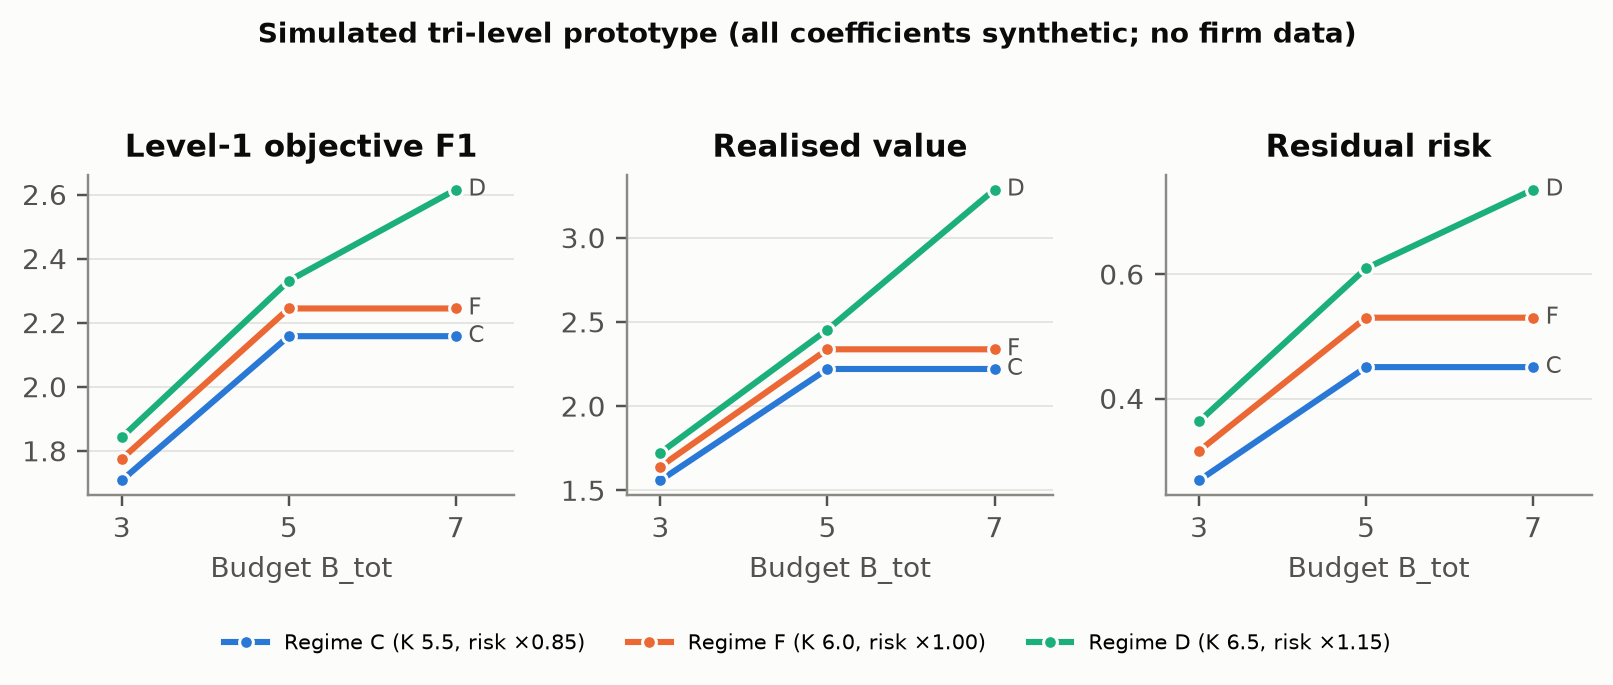
\includegraphics[width=\linewidth]{fig_mlp_scenarios.png}
\caption{Simulated tri-level prototype: Level-1 objective $F_1$, realised value and residual risk by budget $B_{\mathrm{tot}}\in\{3,5,7\}$ for regimes C ($K$ 5.5, risk $\times0.85$), F ($K$ 6.0, risk $\times1.00$) and D ($K$ 6.5, risk $\times1.15$). All coefficients are simulated; no firm data are used, and the outputs do not describe any real firm. Under C and F the budget-7 solution equals the budget-5 solution; under D one process moves to HumanFirstAICheck at budget 7.}
\label{fig:mlp_scenarios}
\end{figure}

The pattern is mechanical and should be read as such. At a budget of 3, every regime leaves one process with HumanOnly and gives two AIAssist. At a budget of 5, all three processes use AIAssist. Under C and F, a budget of 7 yields the same solution as a budget of 5. Under D, one process moves to HumanFirstAICheck, raising $F_1$ to 2.616, realised value to 3.286 and residual risk to 0.736. Within each budget, $F_1$, realised value and residual risk rise from C to F to D. This ordering reflects the regime parameters---larger capacity and flexibility multipliers, but also a larger risk multiplier---not any property of an organisation.

Two probes show the mechanism the model is built to represent. In the \emph{governance permission probe} (regime C, budget 5), withdrawing permission for a configuration lowers $F_1$ from 2.158 to 0.837, and the configurations change from AIAssist $\times3$ to HumanOnly $\times2$ plus HumanFirstAICheck $\times1$. Capabilities and budget are unchanged; the solution is bound by permission, not by capability. This is the distinction Study~3 is designed to observe, and the probe is an illustration of it, not evidence. In the \emph{selection-threshold sensitivity}, process P2 has score 0.65 and a true outcome of 1. At $\tau\leq0.6$ the AI recommendation is correct, and P2 uses AIAssist ($F_1$ 2.244, the value of the regime-F, budget-5 baseline). At $\tau=0.7$ the recommendation is wrong, Level~1 allocates nothing to P2's AI capability, and P2 reverts to HumanOnly ($F_1$ 1.450). A single threshold choice thus propagates upward to the allocation decision. Because the score and the outcome are fixed and known to all levels, the probe shows this propagation only; it says nothing about error rates.

\subsection{Study 3: a preregistered enterprise study (plan, not results)}
\label{sec:mlp_study3}

Study~3 aims to locate where AI--decision integration breaks inside organisations and to calibrate the parameters of the model. The unit of analysis is the decision process, within one or more manufacturing firms; the firm is identified in the thesis and anonymised in this paper. Table~\ref{tab:back_study3} maps the planned data to the model.

\begin{table}[htbp]
\centering
\caption{Study~3 (plan): planned data mapped to model levels and parameters. No data have been collected; no result is reported or implied.}
\label{tab:back_study3}
\footnotesize
\begin{tabular}{p{2.6cm}p{6.2cm}p{5.4cm}}
\toprule
Model level & Planned data & Parameters informed \tabularnewline
\midrule
\raggedright Level 1 & \raggedright AI budgets and staffing by process & \raggedright $b_i^r$, $B_{\mathrm{tot}}$ \tabularnewline
\raggedright Level 2 & \raggedright Approval and audit workflows; decision-rights matrices & \raggedright $\mathrm{Allow}_{m\Gamma}$, $H_{\mathrm{req}}$, $EA_{\mathrm{req}}$, $K_\Gamma$ \tabularnewline
\raggedright Level 3 & \raggedright Process observation and interviews on the configurations actually used & \raggedright $q_{im}$ \tabularnewline
\raggedright Optional organisational structural-hole test & \raggedright De-identified aggregate metadata on tickets and meetings between AI staff and decision owners & \raggedright Burt constraint, assessed against portfolio-style nulls as in Study~2 \tabularnewline
\bottomrule
\end{tabular}
\end{table}

The decision rules will be frozen before data access, as in Study~2 \citep{nosek2018preregistration}. A pattern supports the organisational-bottleneck hypothesis if configurations that are feasible on capability grounds are blocked by permissions ($\mathrm{Allow}_{m\Gamma}$) or by shared capacity ($K_\Gamma$) rather than by capability ceilings. A pattern contradicts it if capability ceilings or data quality bind first. The preregistration will also specify a stop rule. The optional network test applies Burt constraint \citep{burt1992structural} to real organisational ties, the level at which embeddedness arguments locate economic action \citep{granovetter1985economic}, and uses nulls that, like the portfolio-preserving null, hold fixed what each unit is responsible for. A three-expert exercise that translated the AI $\times$ decision categories into enterprise language serves only as a pilot for the instruments, not as evidence. Study~3 tests the hypothesis of Section~\ref{sec:discussion_hypothesis}; it has not been run.

% ------------------------------------------------------------
\section{Limitations}
\label{sec:limitations}

\subsection{Measurement and data}
\label{sec:lim_measurement}

The Study~1 coding has low reliability. Human--human agreement is $\kappa$ 0.05 for AI families and 0.14 for decision families \citep{cohen1960coefficient}, and the depleted cells lose significance under realistic misclassification. The 16 depleted cells are therefore not ``16 statistically robust depleted pairs''; only their direction is defensible. Agreement between two models (0.72 / 0.56) shows reproducibility, not human reliability. The coding also differs in substance between coders: under codebook v2, 42--64\% of evidence sentences state no explicit decision function, against a pipeline rate of 18\%, and only about 9\% of matrix records are reproduced in the same cell by both new coders. Depleted core cells pass the strict filter more often than other cells (38\% vs 28\%), so the filtering step itself may shape the pattern. The V6--V11.1 network results are HISTORICAL / USER\_REPORTED, and their raw files were not re-verified.

In Study~2, CPC classes are proxies for knowledge domains. ``Decision'' is operationalised as G06Q10/04 plus G06Q10/06, broadened to all of G06Q10 only in sensitivity check s2. Label validity rests on a title-keyword lift check (P4), not on a human audit. The relative test H1a depends on the chosen reference set, CPC main groups in G06, G16 and H04, and bridge patents are excluded from the cross counts in the primary specification; counting them on both sides (s6) raises OE to 4.25. Patent citations are an imperfect flow proxy: examiner-added citations are excluded only through PatentsView citation categories \citep{alcacer2006patent,uspto2026patentsview}, and because earlier non-examiner citations are labelled ``cited by other'', the applicant-only specification effectively begins in 2013. The data cover US patents only, and patented inventions rather than organisational practice. Firm identities rely on disambiguated assignees, and the alias check covered 54 firms. Finally, no external organisational source passed the flow-validity gates, and SEC data were not fetched.

\subsection{Inference and design}
\label{sec:lim_inference}

All results are associational; no causal effect is claimed. Failing to support a hole is not proof that none exists under other data, other operationalisations or in other countries. The aggregate rule detected 30\% and 50\% planted suppression in synthetic data, but cell-level power for a 20\% depletion in cells with $E\geq100$ was 67\% (Part~A) and 79\% (Part~B), so weaker depletions or smaller cells may be missed. A domain-level aggregate can also mask heterogeneity; the cell-level analysis addresses this only within the limits of that power. Plans 2--4 were written after earlier results were known. Their decision rules were frozen before computation, but the choice of which follow-up questions to ask was informed by data (Appendix~\ref{app:prereg}).

The preregistered document-preserving null proved degenerate (amendment B1). The M06-P replacement was frozen in the third preregistration before it was run, but it remains a documented deviation from the second plan (Appendix~\ref{app:prereg}). The portfolio null reproduces 85\% (primary) and 91\% (S-tech) of the specialist separation; the remainder is unexplained and is not interpreted as a hole. The P6 cross-weight-retained metric is uninformative by construction. Cell-level patent depletions do not replicate across time halves, and the quantum row is very small (74 edges in Part~A).

\subsection{The model and the organisational hypothesis}
\label{sec:lim_model}

All coefficients of the multi-level model are simulated and uncalibrated; its outputs reflect no real firm. Exact enumeration of a bounded three-process prototype is no evidence of tractability at realistic scale \citep{jeroslow1985polynomial}, and shared follower constraints would require a generalised equilibrium concept rather than the Nash benchmark \citep{nash1951noncooperative}. The conformance check shares its threshold implementations with the solver and cannot by itself detect a common-mode defect in those functions. That the bottleneck is organisational is a hypothesis for Study~3, not a result. Study~3 is planned in one or more manufacturing firms, which will limit generalisation; its instruments have not yet been validated, the optional network test depends on access to de-identified metadata, and the expert translation exercise is a pilot only. Should Study~3 find that capability ceilings or data quality bind first, the hypothesis of Section~\ref{sec:discussion_hypothesis} would be contradicted, and the model's governance layer would need revision.

% ------------------------------------------------------------
\section{Conclusion}
\label{sec:conclusion}

We set out to test, rather than assume, the premise that AI and decision-making are separated by a structural hole. At the level of knowledge domains, the evidence does not support it. US patents in AI and in decision technologies cite each other at about three times the time-stratified expectation (OE 3.05), both preregistered relative criteria fail, and the verdict \texttt{HOLE\_NOT\_SUPPORTED} is stable across all sensitivity specifications. The over-connection is declining but persistent. Cell-level depletions are small and do not replicate over time.

At the firm level, specialist AI and decision firms are less connected than expected, but 85--91\% of that separation is reproduced by a null that preserves firms' portfolios, and mixed-portfolio firms show no brokerage advantage. The preregistered verdict is \texttt{PARTIAL}, and no firm-level structural hole beyond portfolio composition is supported. The literature evidence of Study~1 supports a directional description only, and no network line confirmed a broker.

The methodological lesson is general: co-occurrence is not flow, and a null model must preserve the structure that generates the data. Projections, bipartite matrices, shared vocabulary and model-assigned labels can each produce the appearance of separation or brokerage.

If firms find it hard to integrate AI into decisions, the explanation is therefore unlikely to lie in a missing bridge between knowledge communities. We hypothesise that it lies inside organisations, in resource allocation, decision rights and governance, and human--AI configuration. The tri-level model formalises this hypothesis; its current outputs are simulated. The preregistered Study~3 is designed to calibrate the model and to test whether the hypothesis holds.
